\documentclass[conference]{IEEEtran}
\IEEEoverridecommandlockouts
\usepackage{cite}
\usepackage{amsmath,amssymb}
\usepackage{graphicx}
\usepackage{booktabs}
\usepackage{textcomp}
\usepackage{xcolor}
\usepackage[hidelinks]{hyperref}
\newcommand{\todo}[1]{\textbf{\textcolor{red}{[TODO: #1]}}}

\begin{document}

\title{Multilingual Public Grievance Classifier and Router}

\author{\IEEEauthorblockN{Raj Kesharwani \and Nishchay Gupta \and Ratnesh Singh \and Anant Rawat \and Pratik Roy}
\IEEEauthorblockN{Rahul Kumar \and Saumya Rai \and Md.\ Zaki \and Shashank Shekhar \and Ravindra Kumar}
\IEEEauthorblockA{CS474 Deep Learning, Indian Institute of Information Technology Bhagalpur\\
Instructor: Dr.\ Mehul Kumar}}

\maketitle

\begin{abstract}
Public grievance portals receive complaints in many languages and rely on manual reading and forwarding.
We present a system that classifies a citizen complaint into a department (water, roads, power, sanitation, other),
scores its urgency and sentiment, and routes it to the responsible authority, served through a REST API and a dashboard
with a per-language accuracy report. We compare a TF-IDF logistic-regression baseline with multilingual transformers
fine-tuned with a shared encoder and three task heads. On a held-out split of 150 generated English, Hindi and Marathi complaints, IndicBERT reaches 0.994 department macro-F1, against 0.969 for both the baseline and multilingual BERT; MuRIL reaches only 0.694 under our fixed four-epoch budget because it had not converged. All of these scores come from templated text and overstate real accuracy: the same baseline scores 0.41 on real BBMP complaint phrases.
\end{abstract}

\begin{IEEEkeywords}
grievance redressal, text classification, multilingual NLP, Indian languages, class imbalance, MuRIL
\end{IEEEkeywords}

\section{Introduction}
Citizens lodge hundreds of thousands of civic complaints about water supply, roads, electricity and waste, and platforms such as CPGRAMS
accept them in many languages. Reading, categorising and forwarding each complaint is slow and error-prone, and mistakes delay urgent cases.
This project builds a decision-support prototype that (i) predicts the responsible department, (ii) estimates urgency and sentiment, and
(iii) routes the complaint, while leaving a human able to review the result. Our contributions are: a data pipeline and evaluation protocol
that reports accuracy \emph{per language}; a comparison of a classical baseline with MuRIL, IndicBERT and multilingual BERT;
and a deployed API and dashboard. With a shared budget of four epochs, IndicBERT is the best encoder (department macro-F1 0.994, urgency 0.889, sentiment 1.000), mBERT matches the TF-IDF baseline on department (0.969), and MuRIL lags (0.694) because it was still improving when training stopped. We stress that these figures come from templated data.

\subsection{Problem statement}
Let a complaint be a short text $x$ written in English, Hindi or Marathi. The system must output three labels: a department $y_d \in \{\text{water, roads, power, sanitation, other}\}$,
an urgency level $y_u$ on a four-level ordered scale, and a sentiment $y_s \in \{\text{negative, neutral, positive}\}$. The department decides where the complaint is routed,
the urgency decides how quickly it should be handled, and the sentiment gives the reviewer a quick sense of the citizen's tone.
The practical difficulty is threefold: the languages differ in script and vocabulary, some departments and urgency levels are much rarer than others, and complaints are short and informal.
\subsection{Objectives}
We set five objectives for the project: (1) build a reproducible data pipeline that cleans, labels and splits multilingual complaints; (2) train a strong classical baseline;
(3) fine-tune and compare three multilingual encoders with a shared-encoder, three-head design; (4) report accuracy per language and not only overall, so that weaknesses in a single language are visible;
and (5) deliver the result as an API and a dashboard that a non-technical reviewer can use.

\section{Related Work}
Multilingual encoders for Indian languages include MuRIL~\cite{khanuja2021muril}, trained on 17 Indian languages with transliterated text, and the
IndicBERT family with the IndicCorp corpora and the IndicXTREME benchmark~\cite{kakwani2020indicnlp,doddapaneni2023towards}.
General-purpose baselines are multilingual BERT~\cite{devlin2019bert} and XLM-R~\cite{conneau2020xlmr}.
For complaint text specifically, Singh et al.~\cite{singh2020complaints} identify complaints in Hindi product reviews and address class imbalance
with SMOTE. To our knowledge there is no public, full-text, multilingual, department-labelled grievance corpus for Indian languages, which shapes our data strategy.
Closest to our setting, Beskorovainyi~\cite{beskorovainyi2026appeals} classifies and routes 10{,}000 Russian-language citizen appeals and compares bag-of-words and TF-IDF with SVM, fastText, Word2Vec+LSTM and multilingual BERT on a three-way appeal-type task; BERT is most accurate, yet a smaller LSTM is deployed because of CPU-only hardware and retraining cost. That work is monolingual, predicts appeal type rather than department, urgency or sentiment, and reports a single score.
Our task differs in covering three Indian languages, three prediction targets and a per-language report.
For the shared-encoder design we follow hard parameter sharing, in which hidden layers are shared across tasks and only the output layers are task-specific~\cite{caruana1997multitask,ruder2017overview}.
We did not test whether sharing helps here (Section~\ref{sec:abl}).

\subsection{Multilingual encoders and Indian-language benchmarks}
Pre-trained transformer encoders are the standard starting point for text classification. Multilingual BERT~\cite{devlin2019bert} and XLM-R~\cite{conneau2020xlmr} cover many languages with one shared vocabulary, but Indian languages form a small share of their training data.
MuRIL~\cite{khanuja2021muril} was built specifically for Indian languages and also sees transliterated text, which matters because citizens often type Hindi or Marathi in Roman script.
The IndicBERT family and the IndicNLP and IndicXTREME resources~\cite{kakwani2020indicnlp,doddapaneni2023towards} supply large Indian-language corpora and evaluation tasks.
Because each of these models makes different choices about data and vocabulary, a direct comparison on one task is informative, and that is what we do here.
\subsection{Complaint and appeal classification}
Work on citizen text is limited, and most of it is not multilingual. Beskorovainyi's appeal classifier~\cite{beskorovainyi2026appeals} shows that, in a government setting, the most accurate model is not always the one deployed:
a smaller network was chosen for its low retraining cost on CPU-only hardware. This reminds us to report not only accuracy but also what each model costs to train and serve.
Singh et al.~\cite{singh2020complaints} detect complaints in Hindi product reviews, which is a different task from routing but is the closest Hindi complaint work we found; they also treat class imbalance, which is central for us.
\subsection{Multi-task learning and class imbalance}
Sharing an encoder across related tasks can act as a regulariser, because the shared representation must serve all tasks at once~\cite{caruana1997multitask,ruder2017overview}.
Department, urgency and sentiment are related, since an angry, urgent complaint about a power cut is both negative and urgent.
Class imbalance is handled in our work by inverse-frequency class weights in the loss, a simple method that needs no resampling of the data.
\subsection{Gap addressed by this work}
We did not find a public benchmark that combines Indian-language complaints, department labels, urgency and sentiment. Our contribution is therefore an end-to-end, reproducible pipeline and an honest per-language comparison on a small dataset, together with a clear statement of how far its numbers can be trusted.

\section{Data}
\subsection{Sources}
We use several sources, each with limits (Table~\ref{tab:data}). The BBMP (Bengaluru) grievance export~\cite{bbmp} has 1.23M rows but only 187 distinct
complaint phrases, because the text field is a sub-category label; we use it for exploratory analysis and as a real-text check.
IndicSentiment~\cite{doddapaneni2023towards} provides 15{,}002 labelled reviews in 13 languages and is used only for sentiment.
Because no source offers full-text multilingual complaints with department labels, we generated 1{,}000 English, Hindi and Marathi complaints
from hand-written sentence templates (issue, location, duration, closing line), with urgency following issue severity.
IndicSentiment was downloaded from Hugging Face (\texttt{ai4bharat/IndicSentiment}) and converted, but it is not yet part of the training data.
We generated the complaints because we found no public, full-text, multilingual, department-labelled grievance corpus: BBMP carries only category labels, IndicSentiment has no departments, one candidate corpus requires a paid subscription, and BanglaPSG is Bangla. Generation lets us build and compare models end to end, at the cost of inflated scores on templated text.
All generated rows are marked \texttt{label\_source=generated}. We did not use team-collected complaints in the experiments reported here, and BanglaPSG~\cite{banglapsg} is Bangla and so outside our three languages.

\begin{table}[t]
\caption{Data sources and how they are used.}
\label{tab:data}
\centering
\small
\begin{tabular}{@{}p{2.1cm}p{1.1cm}p{4.2cm}@{}}
\toprule
Source & Size & Role and limitation \\
\midrule
Generated (en/hi/mr) & 1{,}000 & Training base; templated wording \\
BBMP export & 187 phrases & Real-text check; no free text \\
IndicSentiment & 15{,}002 & Sentiment only; reviews, no neutral \\
\bottomrule
\end{tabular}
\end{table}

\subsection{Label definitions}
\emph{Department} has five classes: water, roads, power, sanitation and other, where ``other'' collects complaints that fit none of the four named authorities.
\emph{Urgency} has four ordered levels, assigned from the severity of the issue and raised by a long duration or an urgent closing line.
\emph{Sentiment} has three classes (negative, neutral, positive); generated rows include neutral and positive examples so that all three classes appear in training.
Every row carries a \texttt{label\_source} tag: \texttt{gold} for labels supplied by a source, \texttt{weak} for keyword-rule labels, and \texttt{generated} for template-built rows.
\subsection{How the generated complaints were built}
A complaint is assembled from four parts: an issue sentence chosen from a hand-written list for one department and severity level, an optional location, a duration, and a closing line that is plain, urgent or angry.
The generator draws these parts at random with a fixed seed, removes duplicate texts, and writes the department, urgency and sentiment that follow from the chosen parts.
This guarantees correct labels and balanced coverage of every department and language, which is why we could build and compare models quickly, but it also means the wording is far less varied than real complaints.

\subsection{Cleaning, labels and splits}
Texts are normalised (URLs and whitespace removed); empty, very short and duplicate texts are dropped; language is detected by script;
missing urgency and sentiment labels are filled by keyword rules and flagged as weak. Data are split 70/15/15 into train, validation and test,
stratified by department with seed 42. The final dataset has 1{,}000 rows (700 train, 150 validation, 150 test) and no row was dropped. Language counts are 420 English, 300 Hindi and 280 Marathi. Department counts are 224 sanitation, 223 roads, 204 power, 199 water and 150 other. The test split has 51 English, 62 Hindi and 37 Marathi complaints.

\subsection{Exploratory analysis}
Figure~\ref{fig:dist} shows the final dataset. The three languages are represented in a 42\%, 30\% and 28\% split, and the four named departments each hold between 199 and 224 rows, with ``other'' at 150.
The classes are therefore only mildly imbalanced in the generated data, and the real-world imbalance we expect (for example, many more road and sanitation complaints than rare categories) is not captured.
A correlation check between department and urgency gave a very weak association (Cram\'er's V about 0.04), while urgency and sentiment were associated (about 0.49); this link is an artefact of how the generator ties the closing line to both labels and should not be read as a property of real complaints.
\begin{figure}[t]
\centering
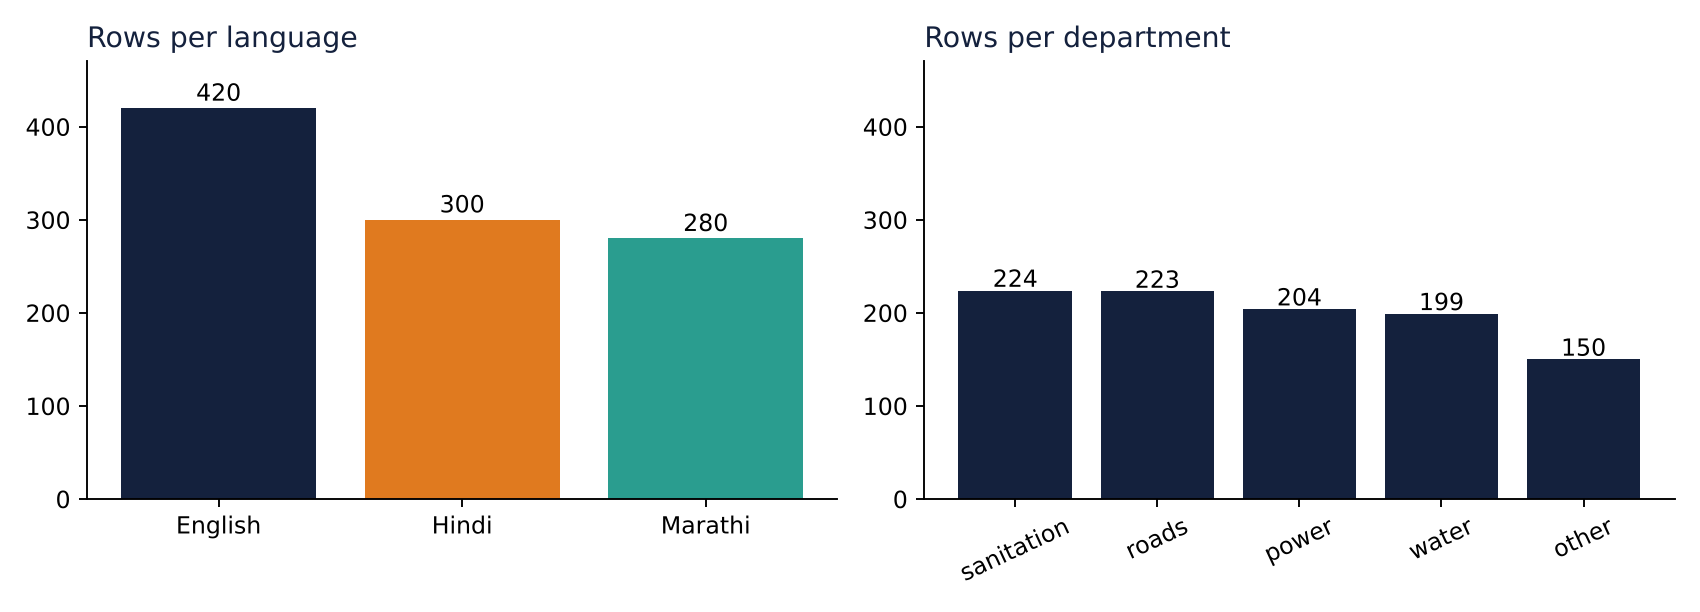
\includegraphics[width=\columnwidth]{figures/data_distribution.png}
\caption{Rows per language and per department in the generated dataset (1{,}000 rows).}
\label{fig:dist}
\end{figure}
\subsection{Privacy and ethics}
Real complaints can contain names, addresses and phone numbers. We use only public, aggregated or generated text, strip identifiers during cleaning, and do not store personal data.
The generated rows contain invented locations and no real individuals. Any future collection of real complaints should obtain consent, remove identifiers, and be reviewed by the team before use.

\section{Method}
\subsection{Problem formulation}
Given a complaint $x$, the model produces three probability distributions, $p_d(x)$, $p_u(x)$ and $p_s(x)$, over departments, urgency levels and sentiments, and the predicted label for each task is the most probable class.
The predicted department is mapped to a responsible authority through a fixed routing table, so routing quality depends directly on department accuracy.
Figure~\ref{fig:arch} shows the architecture used for the transformer models.
\begin{figure}[t]
\centering
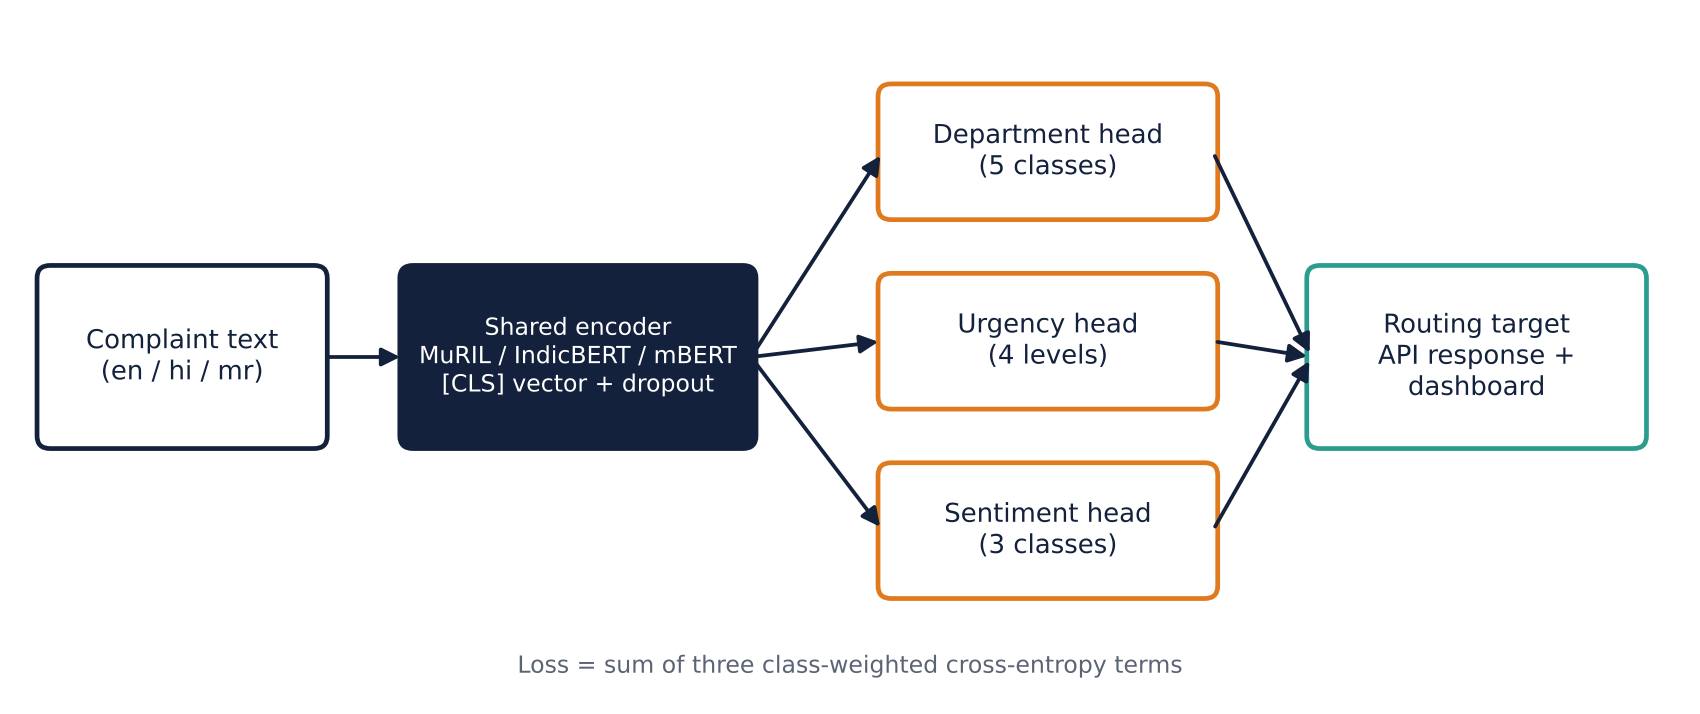
\includegraphics[width=\columnwidth]{figures/architecture.png}
\caption{Multitask architecture: one shared encoder and three task heads, trained with a summed, class-weighted loss.}
\label{fig:arch}
\end{figure}

\subsection{Baseline}
TF-IDF features over word 1--2-grams with a class-weighted logistic regression predict the department; urgency and sentiment come from keyword rules.
\subsection{Encoders compared}
We compare three pre-trained encoders under identical settings.
\textbf{MuRIL} (\texttt{google/muril-base-cased}) is trained on 17 Indian languages and includes transliterated text~\cite{khanuja2021muril}.
\textbf{IndicBERT v2} (\texttt{ai4bharat/IndicBERTv2-MLM-only}) comes from the IndicCorp and IndicXTREME effort~\cite{kakwani2020indicnlp,doddapaneni2023towards}.
\textbf{mBERT} (\texttt{bert-base-multilingual-cased}) is the general-purpose multilingual baseline~\cite{devlin2019bert}.
All three are 12-layer base-size BERT encoders, so the comparison isolates the pre-training data and vocabulary rather than model size.
\subsection{Multitask transformer}
A pre-trained encoder (MuRIL, IndicBERT or mBERT) feeds the [CLS] representation through dropout to three linear heads (department, urgency, sentiment).
The loss is the sum of three cross-entropy terms with inverse-frequency class weights (absent classes get weight zero), optimised with AdamW and a linear warm-up schedule;
the epoch with the best validation department macro-F1 is kept. All three encoders use the same settings: learning rate $3{\times}10^{-5}$, batch size 16, 4 epochs, maximum length 128 tokens and seed 42, with class weighting on.
\subsection{Loss and class weighting}
For task $t \in \{d,u,s\}$ with $K_t$ classes, $N_t$ training examples and $n_{t,c}$ examples of class $c$, the weight of class $c$ is
\begin{equation}
w_{t,c} = \frac{N_t}{K_t \, n_{t,c}},
\end{equation}
and $w_{t,c}=0$ when class $c$ does not occur in the training data, so an absent class cannot cause a division by zero. The total loss is the sum of the three weighted cross-entropy terms,
\begin{equation}
\mathcal{L} = \sum_{t \in \{d,u,s\}} \frac{1}{B}\sum_{i=1}^{B} w_{t,y_{t,i}} \bigl(-\log p_t(y_{t,i}\mid x_i)\bigr),
\end{equation}
where $B$ is the batch size. Rare classes thus contribute more per example, which discourages a model from always predicting the majority class.
\subsection{Training procedure}
Each run fine-tunes all encoder parameters together with the three linear heads using AdamW and a linear warm-up schedule, with the settings of Section~\ref{sec:setup}.
After every epoch we compute the validation department macro-F1 and keep the checkpoint with the highest value, so a late, worse epoch cannot replace a better one.
A run writes its metrics, per-language report and confusion matrix to a folder named after the model, so every number in this paper can be traced to a file.

\subsection{System}
A FastAPI service exposes single and batch prediction, and a Streamlit dashboard supports pasting or uploading complaints and shows the per-language report.
Predictions include the routing target for the predicted department.

\section{System Implementation}
The prediction code is shared by two front ends. A FastAPI service exposes \texttt{/health} for liveness, \texttt{/model} for the loaded model's details, \texttt{/predict} for one complaint and \texttt{/predict/batch} for many.
Empty or invalid text returns a validation error (HTTP 422), and a request made when no model is loaded returns a service-unavailable error (HTTP 503), so failures are explicit.
Which model is served is chosen by an environment variable pointing at a fine-tuned model folder; if it is not set, the TF-IDF baseline is served, so the service always starts.
A Streamlit dashboard lets a reviewer paste or upload complaints and shows the predicted department, urgency, sentiment and routing target, together with the per-language accuracy report.
A Docker image packages the baseline API for deployment. The repository includes 39 automated tests that cover the data pipeline, the models, the API and the importers, and they all pass.

\section{Experiments}
\subsection{Setup}\label{sec:setup}
We report accuracy and macro-F1 per task and per language, the department confusion matrix, and error analysis. Because generated text is templated,
we also evaluate on real text kept out of training. All models were fine-tuned on a single free Google Colab GPU (T4) with one seed (42), so we report no variance across seeds and small differences should not be over-read.
\subsection{Metrics}
\emph{Accuracy} is the fraction of complaints labelled correctly. \emph{Macro-F1} averages the per-class F1 score, where F1 is the harmonic mean of precision and recall, giving every class equal weight so that a poorly handled small class lowers the score.
We use macro-F1 as the main metric because accuracy can look high while a small class is ignored. A \emph{confusion matrix} counts, for each actual department, how many complaints were assigned to each predicted department.
All three metrics are computed on the held-out test split only, and the \emph{per-language report} repeats them separately for English, Hindi and Marathi.
\subsection{Protocol}
All models see the same 700 training, 150 validation and 150 test complaints. The validation set is used only to choose the best epoch, and the test set is used once per model for the reported numbers.
The same settings are used for every encoder so that differences come from the encoder and not from tuning.

\subsection{Ablations}
\label{sec:abl}
We ran two ablations: the choice of encoder (MuRIL, IndicBERT, mBERT) and class weighting on versus off for MuRIL. We did not run single-task versus multitask, generated-only versus generated plus real data, or training with IndicSentiment; these remain future work.

\section{Results}
Table~\ref{tab:baseline} gives the baseline. On the generated test split it scores very high because the text is templated, and it falls sharply on real BBMP phrases,
so we treat the real-text figure as the more honest indicator (Fig.~\ref{fig:real}).

\begin{figure}[t]
\centering
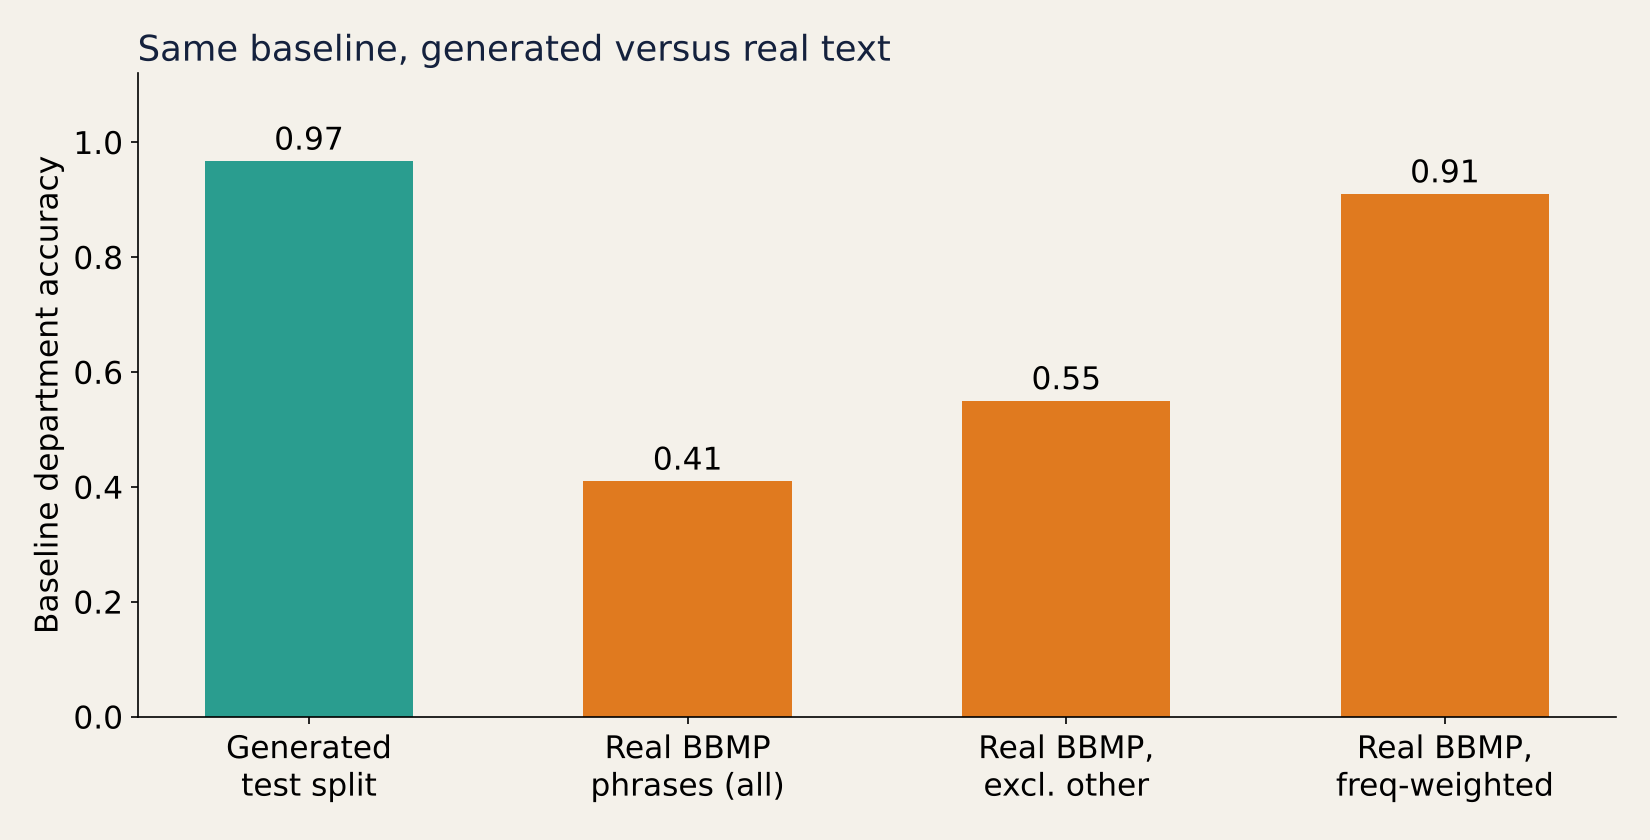
\includegraphics[width=\columnwidth]{figures/real_vs_gen.png}
\caption{Baseline accuracy on the generated test split versus real BBMP phrases.}
\label{fig:real}
\end{figure}

\begin{table}[t]
\caption{Baseline department classification (TF-IDF + logistic regression).}
\label{tab:baseline}
\centering
\small
\begin{tabular}{@{}lcc@{}}
\toprule
Evaluation set & Accuracy & Macro-F1 \\
\midrule
Generated test split ($n{=}150$) & 0.967 & 0.969 \\
BBMP phrases, all ($n{=}186$) & 0.41 & -- \\
BBMP phrases, excl.\ ``other'' ($n{=}38$) & 0.55 & -- \\
BBMP, excl.\ ``other'', frequency-weighted & 0.91 & -- \\
\bottomrule
\end{tabular}
\end{table}

Keyword rules reach 0.473 accuracy on urgency and 0.233 on sentiment on the generated test split and never predict positive sentiment, so trained heads are required.
Table~\ref{tab:models} compares the models on the generated test split. IndicBERT is best on department and sentiment; mBERT is best on urgency. The baseline has no trained urgency or sentiment head.

\begin{figure}[t]
\centering
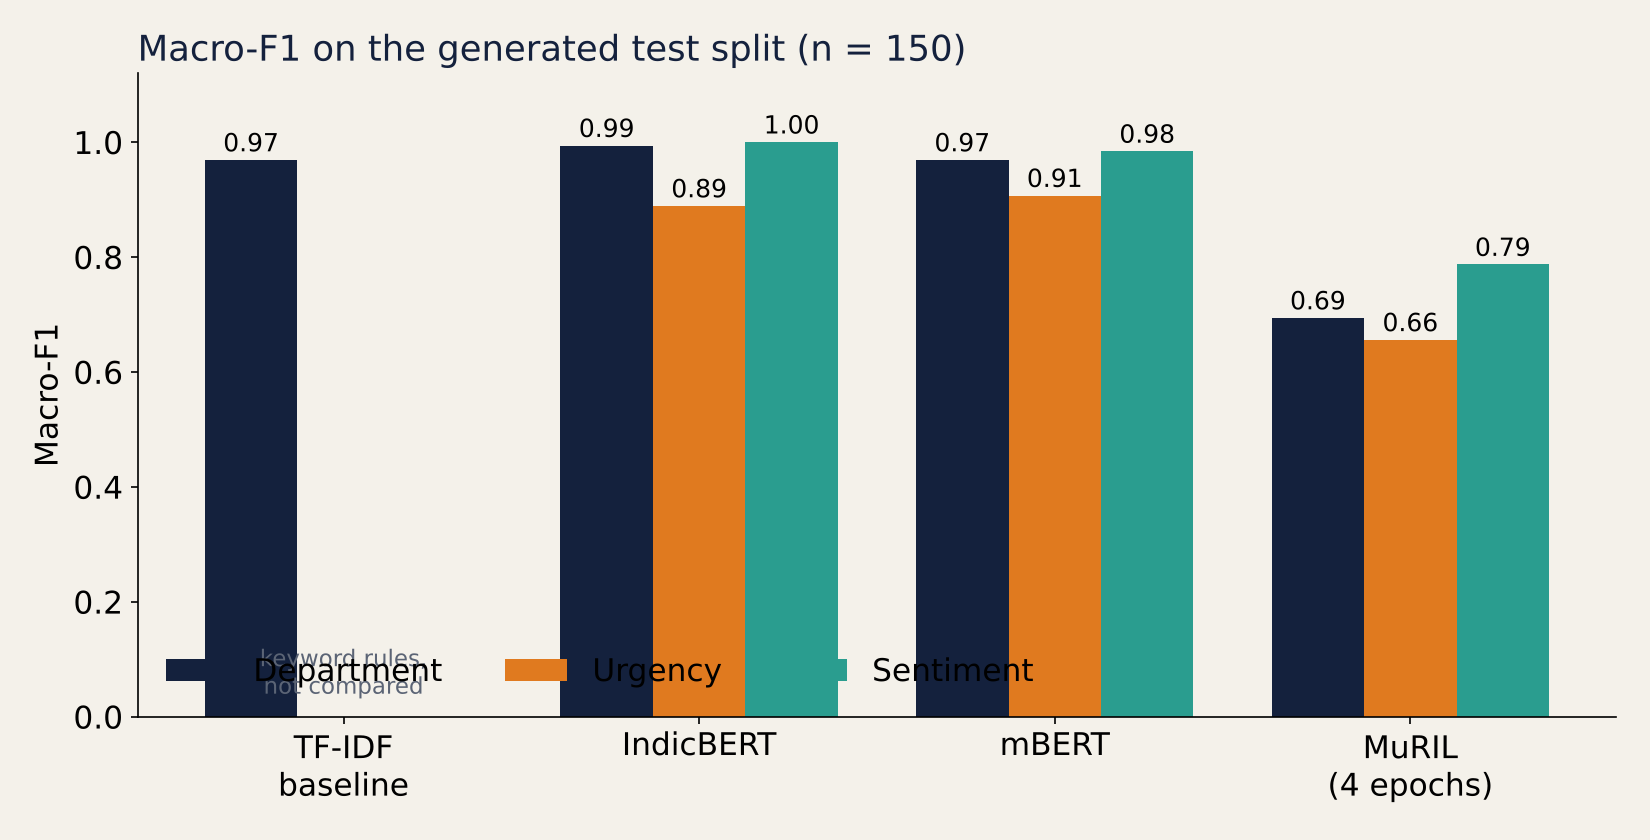
\includegraphics[width=\columnwidth]{figures/models.png}
\caption{Macro-F1 per task for each model on the generated test split.}
\label{fig:models}
\end{figure}

\begin{table}[t]
\caption{Macro-F1 on the generated test split ($n{=}150$). Baseline urgency and sentiment use keyword rules and are omitted.}
\label{tab:models}
\centering
\small
\begin{tabular}{@{}lccc@{}}
\toprule
Model & Dept. & Urgency & Sentiment \\
\midrule
TF-IDF + LogReg & 0.969 & -- & -- \\
IndicBERT & \textbf{0.994} & 0.889 & \textbf{1.000} \\
mBERT & 0.969 & \textbf{0.907} & 0.984 \\
MuRIL & 0.694 & 0.656 & 0.787 \\
MuRIL, no class weights & 0.074 & 0.153 & 0.310 \\
\bottomrule
\end{tabular}
\end{table}

Table~\ref{tab:lang} gives department macro-F1 per language (Fig.~\ref{fig:lang}). Hindi is the weakest language for the baseline (0.929) and IndicBERT (0.985), and Marathi for mBERT (0.931). MuRIL is weakest on Marathi (0.536).

\begin{table}[t]
\caption{Department macro-F1 per language on the test split.}
\label{tab:lang}
\centering
\small
\begin{tabular}{@{}lccc@{}}
\toprule
Model & en ($n{=}51$) & hi ($n{=}62$) & mr ($n{=}37$) \\
\midrule
TF-IDF + LogReg & 1.000 & 0.929 & 1.000 \\
IndicBERT & 1.000 & 0.985 & 1.000 \\
mBERT & 1.000 & 0.969 & 0.931 \\
MuRIL & 0.746 & 0.713 & 0.536 \\
\bottomrule
\end{tabular}
\end{table}

\begin{figure}[t]
\centering
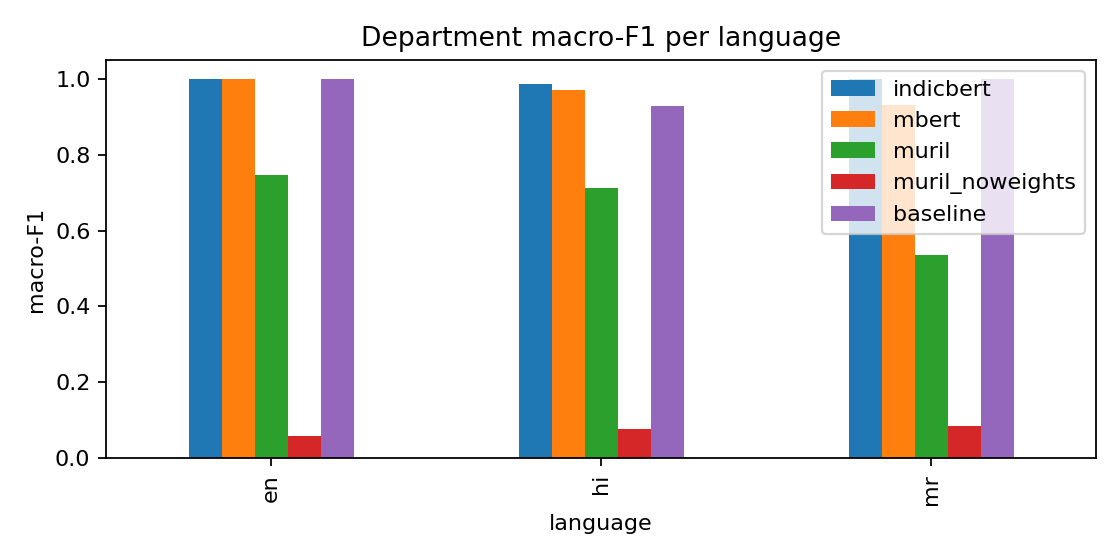
\includegraphics[width=\columnwidth]{figures/per_language_f1.png}
\caption{Department macro-F1 per language.}
\label{fig:lang}
\end{figure}

\subsection{Why IndicBERT scored best}
IndicBERT obtained the highest department macro-F1 (0.994) and the highest sentiment macro-F1 (1.000), with one department error in 150 test complaints.
We did not run experiments that isolate the cause, so the following explanations are hypotheses and not findings.
First, IndicBERT is pre-trained on text in Indian languages, which may suit Hindi and Marathi complaints better than mBERT, whose training data covers many languages with less Indian-language text.
Second, IndicBERT trained stably within four epochs under a learning rate of $3{\times}10^{-5}$, reaching a validation macro-F1 of 1.00, while MuRIL's validation score was still rising at epoch four, so MuRIL's low score reflects an unfinished fit and not evidence that it is a weaker model.
Third, the test split is templated, so several models can do well and small differences are not statistically reliable with one seed.
mBERT was best on urgency (0.907), which shows no single encoder dominated every task.
\begin{figure}[t]
\centering
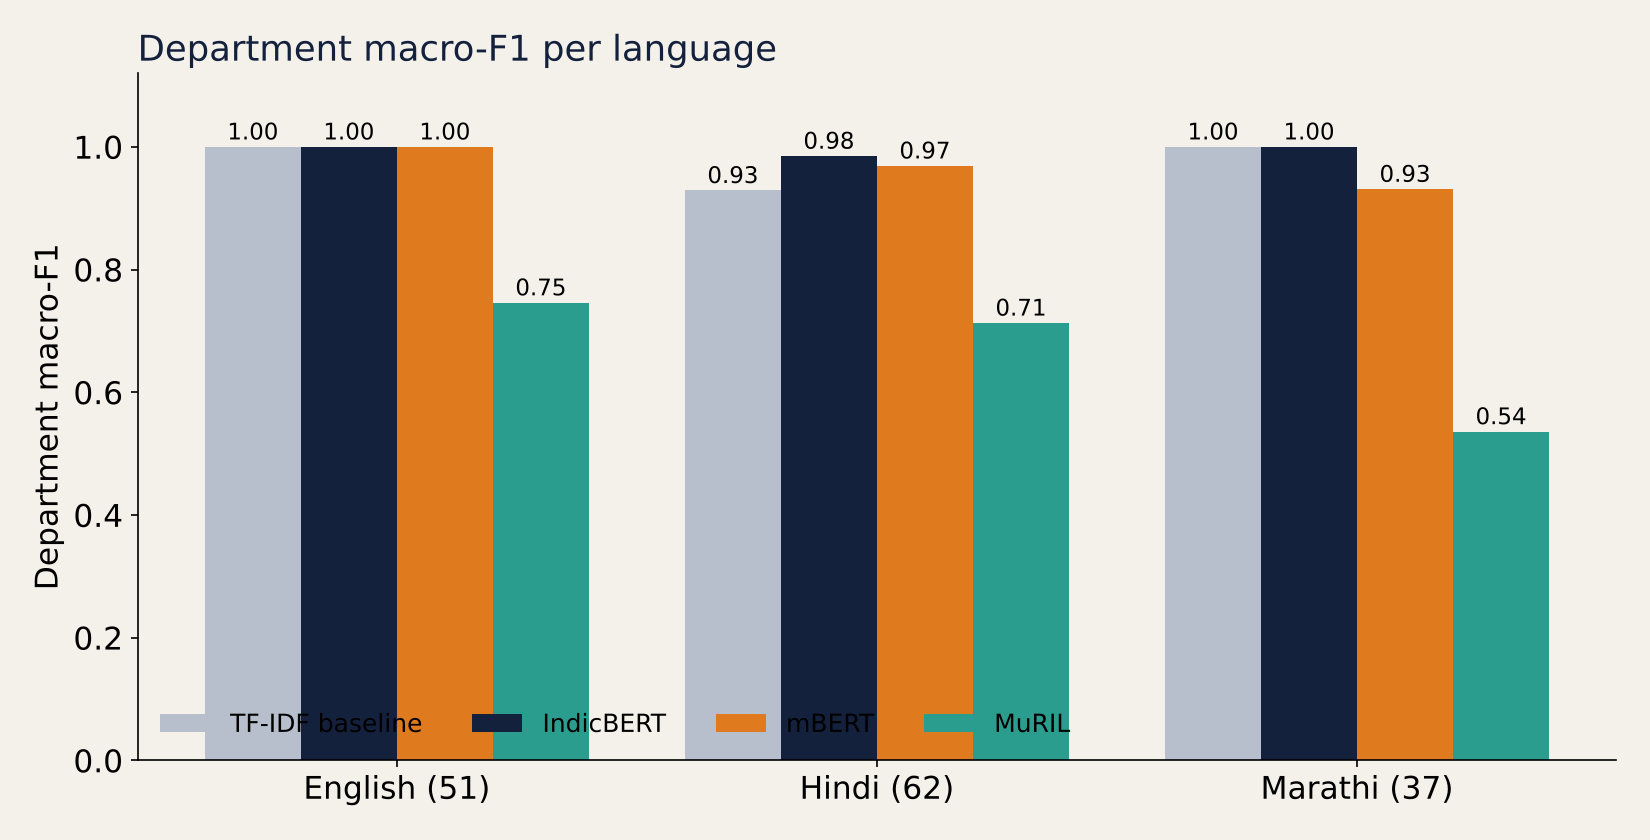
\includegraphics[width=\columnwidth]{figures/per_language_chart.png}
\caption{Department macro-F1 per language for the baseline and the three encoders.}
\label{fig:perlang2}
\end{figure}
\begin{table}[t]
\caption{Full test metrics: accuracy / macro-F1 for each task ($n{=}150$).}
\label{tab:full}
\centering
\footnotesize
\begin{tabular}{@{}lccc@{}}
\toprule
Model & Department & Urgency & Sentiment \\
\midrule
TF-IDF + LogReg & 0.967 / 0.969 & -- & -- \\
IndicBERT & 0.993 / 0.994 & 0.880 / 0.889 & 1.000 / 1.000 \\
mBERT & 0.967 / 0.969 & 0.913 / 0.907 & 0.993 / 0.984 \\
MuRIL & 0.687 / 0.694 & 0.733 / 0.656 & 0.893 / 0.787 \\
MuRIL, no weights & 0.227 / 0.074 & 0.440 / 0.153 & 0.867 / 0.310 \\
\bottomrule
\end{tabular}
\end{table}

\subsection{Per-task observations}
\emph{Department.} The baseline, mBERT and IndicBERT all reach at least 0.969 macro-F1, so on templated text the department task is nearly saturated and a bag-of-words model is already strong.
\emph{Urgency.} Urgency is harder than department for every transformer (0.889 for IndicBERT and 0.907 for mBERT), because it depends on severity and duration cues that are spread across the sentence and not on a few keywords.
\emph{Sentiment.} Sentiment is almost perfect for IndicBERT and mBERT (1.000 and 0.984), which is expected because the generated closing lines carry clear sentiment cues; this is not evidence that real sentiment would be as easy.
Since urgency and sentiment labels for generated rows come from rules, high scores on these tasks measure agreement with those rules and not human judgement.
\emph{Languages.} English is solved by all models except MuRIL. Hindi and Marathi separate the models, which supports our decision to report accuracy per language.

\subsection{Error analysis}
Figure~\ref{fig:cm} shows the department confusion matrices. IndicBERT makes one error in 150 (a sanitation complaint predicted as water), and mBERT makes five (water and power complaints predicted as roads, and one sanitation as water). MuRIL's errors are systematic: 14 of 33 sanitation complaints are predicted as roads, 8 of 23 ``other'' complaints as roads, and 7 of 30 power complaints as roads, so it collapses toward the roads class.
Its validation macro-F1 rose from 0.07 to 0.28, 0.55 and 0.69 over the four epochs and was still increasing, so these errors reflect an unfinished fit and not a limit of the encoder.
Without class weights MuRIL stayed at 0.072 validation F1 for all four epochs, but because MuRIL itself is undertrained this does not isolate the effect of weighting.
Figure~\ref{fig:curve} shows the MuRIL validation curve.
We did not export misclassified complaint texts for the transformers, so we give no per-example analysis.

\begin{figure}[t]
\centering
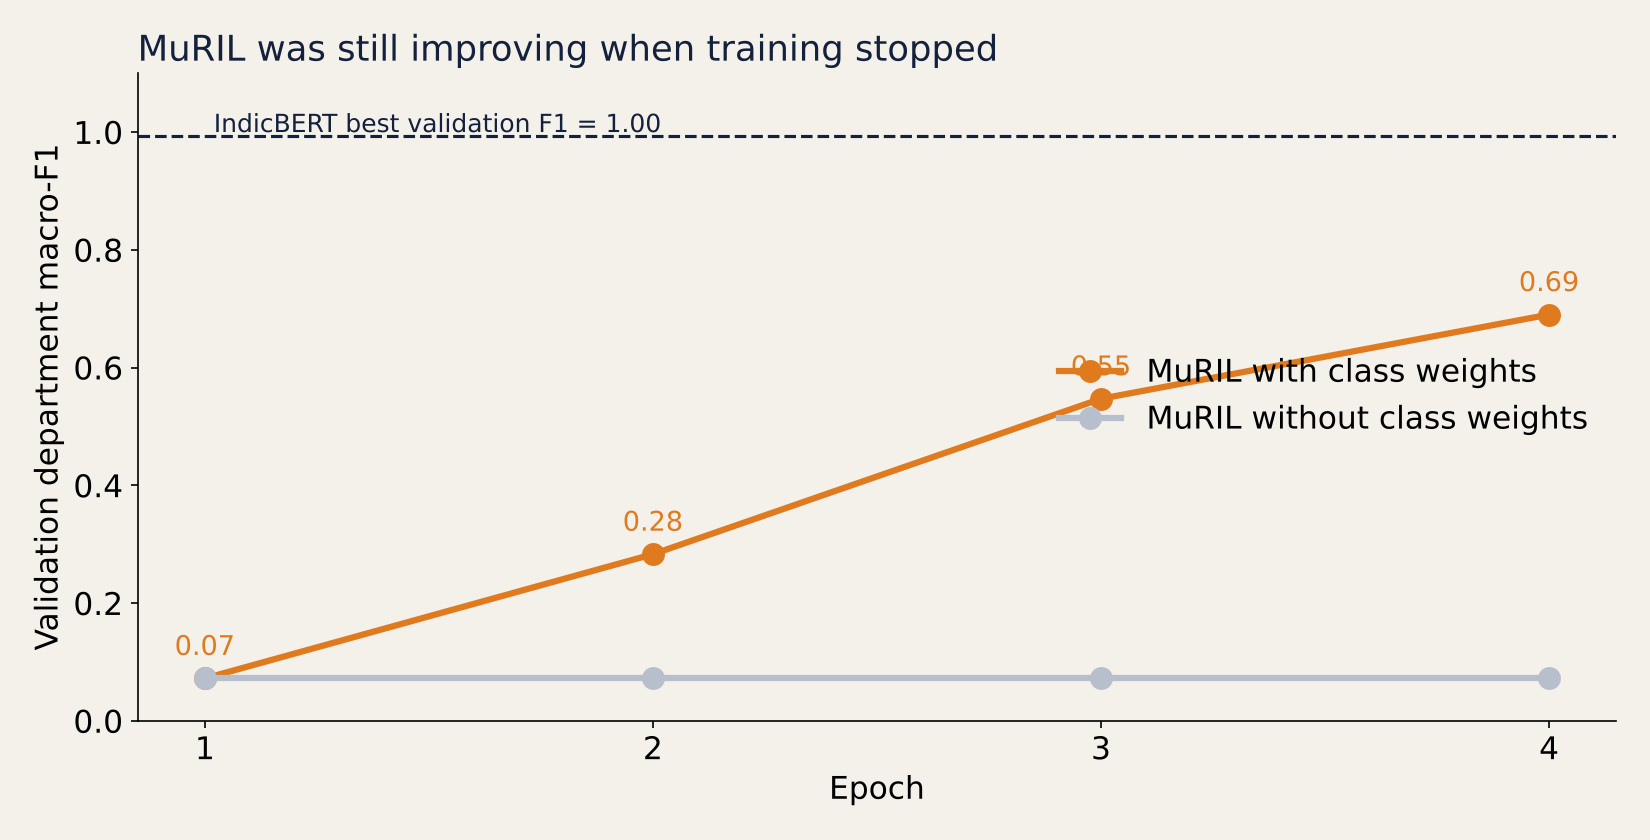
\includegraphics[width=\columnwidth]{figures/muril_curve.png}
\caption{MuRIL validation department macro-F1 per epoch, with and without class weights.}
\label{fig:curve}
\end{figure}

\begin{figure}[t]
\centering
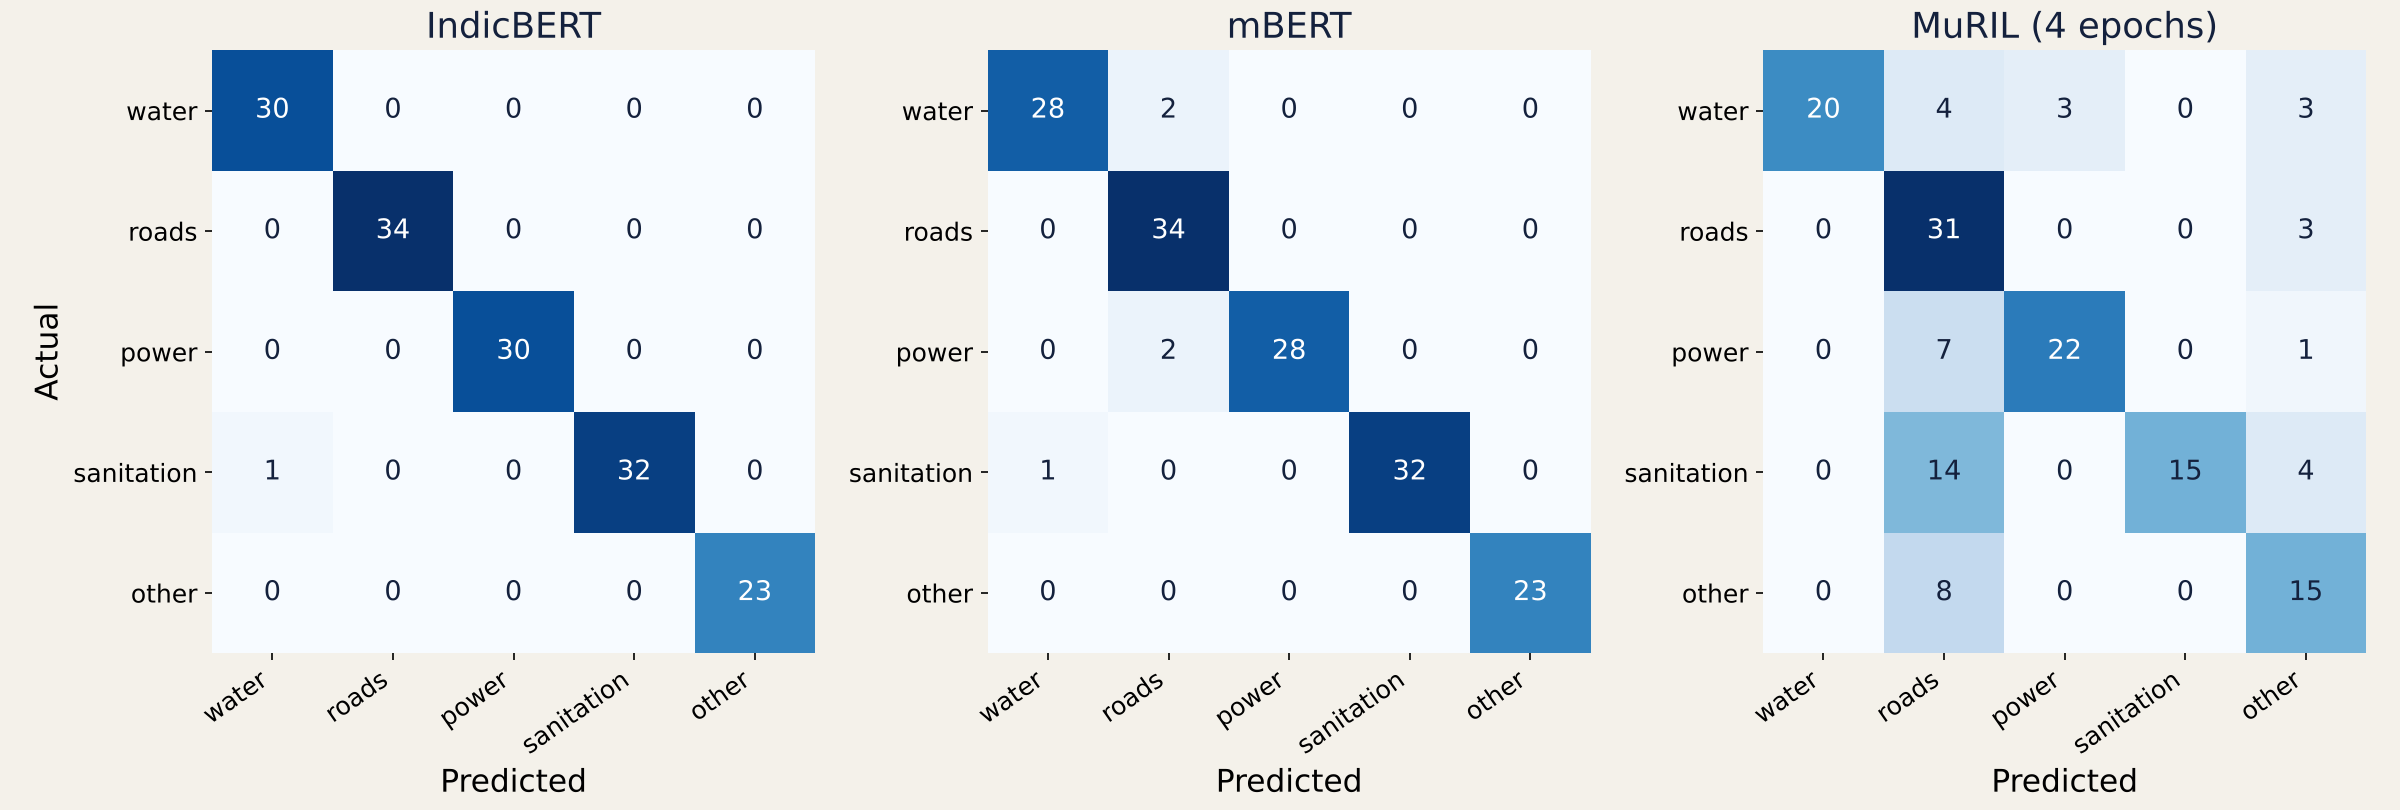
\includegraphics[width=\columnwidth]{figures/confusion_matrices_all.png}
\caption{Department confusion matrices for the three transformers (rows actual, columns predicted).}
\label{fig:cm}
\end{figure}

\section{Discussion and Limitations}
Generated complaints are templated, so high scores on a generated split overstate real-world accuracy. The BBMP check is small and its category-to-department mapping is noisy.
Language coverage is uneven, and Hindi and Marathi sentences were written without full native-speaker review.
Complaints may contain personal details; we use only public, anonymized data and strip identifiers. The system is a decision-support prototype: a person should be able to review
and override routing, especially for critical urgency. In the transformer experiments, the gap between IndicBERT and mBERT (0.994 vs 0.969) is five errors versus one in 150 examples from a single seed, which is too small to rank them confidently. MuRIL, the encoder designed for Indian languages, scored lowest, but only because it had not converged in four epochs; a fair comparison needs longer training or a higher learning rate. The very high scores of the other models show that the templated task is easy, not that routing is solved.

\subsection{Real-text evaluation of the baseline}
To check how far the generated-data scores transfer, we scored the baseline on the 186 distinct BBMP complaint phrases, mapping each BBMP category to one of our departments (for example, electrical to power, solid waste and sanitation to sanitation, road maintenance and road infrastructure to roads, storm water drain and water crisis to water, and every other category to ``other'').
Accuracy was 0.41 over all phrases and 0.55 over the 38 phrases that are not ``other''; weighted by how often each phrase occurs in the export, accuracy on non-``other'' phrases was 0.91, because the common complaint types are the easy ones.
Two causes explain the drop: the phrases are short category-style labels, unlike our full-sentence templates, and the category-to-department mapping is itself approximate, so some ``errors'' are label noise.
We did not run the fine-tuned transformers on these phrases, so we cannot say whether they transfer better; this is the first thing to test.
\subsection{Limits of keyword-rule labels}
Urgency and sentiment labels for rows without a source label come from keyword rules. These rules are transparent and cheap, but they never predict positive sentiment on their own and reach only 0.473 accuracy on urgency and 0.233 on sentiment as classifiers on the generated test split,
which is why trained heads are needed. The trained heads, however, learn from labels that the same rules or templates produced, so their scores reflect agreement with those rules.
Human-labelled urgency and sentiment for a sample of real complaints would be the most valuable addition to the dataset.
\subsection{Practical use and human oversight}
In a real grievance office the model should assist, not replace, a human reader. We recommend showing the predicted department with its confidence, letting a reviewer override the routing, and sending low-confidence or critical-urgency complaints to manual review.
The transformer predictor returns a confidence for each task, which supports such a threshold. Errors are not equally costly: sending an urgent power-failure complaint to the wrong department delays help, while mislabelling a neutral comment matters little.
\subsection{Cost and efficiency}
The baseline trains in seconds on a CPU and can be served in a small container, while each transformer needs a GPU for fine-tuning and a larger serving image.
Following the lesson of deployed appeal classifiers~\cite{beskorovainyi2026appeals}, a team should weigh the accuracy gain of a transformer against its training and serving cost.
On our templated data the baseline matches mBERT on department (0.969) at a fraction of the cost, so the extra cost is justified only if gains also appear on real text, which we have not yet measured.

\subsection{Threats to validity}
\emph{Construct validity:} the labels for generated rows are produced by the same templates that produce the text, so the model can learn the generator's habits instead of real language understanding.
\emph{Internal validity:} each model was trained once with a single seed, so a difference of one or two errors in 150 examples may be chance. \emph{External validity:} the real-text check uses only 186 short BBMP phrases in English, so we have no real Hindi or Marathi evidence at all.
We therefore regard the numbers as a demonstration that the pipeline works and as a relative comparison on templated data, not as an estimate of deployed accuracy.
\subsection{Reproducibility}
The repository fixes the seed to 42, stores each model's settings in a YAML file, and provides scripts that regenerate the data, train the baseline and each encoder, and build the results table.
A notebook runs the whole experiment on a free GPU and produces a downloadable results archive, and the data card records how many rows were read, dropped and kept, per language and department.
\subsection{Team contributions}
The 10-member team was organised into data (two members), modelling (three), evaluation (two), deployment (two) and coordination (one), following the split recommended in the course brief, with each member expected to commit weekly to a shared repository.

\section{Conclusion}
We built a pipeline, a multitask model, an API and a dashboard for classifying and routing multilingual grievances, and a per-language evaluation. On generated data IndicBERT scored best (department macro-F1 0.994), mBERT matched the TF-IDF baseline (0.969), and MuRIL was undertrained (0.694). The more important result is the gap between templated and real text: the baseline falls to 0.41 on real BBMP phrases. Future work is to collect and label real Hindi and Marathi complaints for an honest test set, train MuRIL to convergence, run the multitask and class-weighting ablations on every encoder with several seeds, replace keyword-rule urgency and sentiment labels with human labels, and keep a person in the loop for critical cases.

\appendix
\subsection{Hyper-parameters}
\begin{table}[h]
\caption{Settings shared by all transformer runs.}
\label{tab:hp}
\centering
\small
\begin{tabular}{@{}ll@{}}
\toprule
Setting & Value \\
\midrule
Learning rate & $3{\times}10^{-5}$ \\
Batch size & 16 \\
Epochs & 4 \\
Maximum length & 128 tokens \\
Optimiser & AdamW, linear warm-up \\
Class weighting & inverse frequency \\
Random seed & 42 \\
Model selection & best validation department macro-F1 \\
\bottomrule
\end{tabular}
\end{table}
\subsection{Repository structure}
The repository separates source code, scripts, configurations, data, results and documents. The package under \texttt{src/grievance} holds the label definitions, the data pipeline and generator, the baseline, the multitask model, the class-weight utilities, the two predictors, the API and the dashboard.
The \texttt{scripts} folder holds the commands for data generation, preparation, training, evaluation and comparison; \texttt{configs} holds one YAML file per encoder; \texttt{reports} holds each run's metrics, per-language report and confusion matrix;
\texttt{docs} holds the data card description, work plan, proposal, experiment log, milestones and this report; and \texttt{tests} holds the automated tests.
\subsection{Project timeline}
\begin{table}[h]
\caption{Course milestones and the matching project artefacts.}
\label{tab:time}
\centering
\footnotesize
\begin{tabular}{@{}p{1.0cm}p{2.7cm}p{3.6cm}@{}}
\toprule
Week & Milestone & Artefact in this repository \\
\midrule
4 & Proposal & \texttt{docs/PROPOSAL.md} \\
6 & Data and baseline & EDA notebook, baseline metrics \\
8 & Mid-term review & Fine-tuned models, results table, slides \\
10 & Improved models & Experiment log, ablations \\
12 & Deployment & API and dashboard \\
13 & Final report & This report and the repository \\
\bottomrule
\end{tabular}
\end{table}

\subsection{Planned follow-up work}
Planned but not yet done: retraining MuRIL for 10 epochs at a learning rate of $5{\times}10^{-5}$; repeating the class-weighting ablation on IndicBERT; running several seeds; collecting and labelling real Hindi and Marathi complaints for testing;
exporting misclassified complaints for error analysis; training with IndicSentiment for the sentiment head; and hosting the API and dashboard for a live demonstration.

\section*{Acknowledgment}
We thank Dr.\ Mehul Kumar and the teaching staff of CS474 for guidance, and Google Colab for free GPU compute.

\bibliographystyle{IEEEtran}
\bibliography{references}

\end{document}
